%! Author = denis
%! Date = 12.06.2026

% Preamble
\documentclass[11pt]{article}

% Packages
\usepackage{amsmath}
\usepackage{graphicx}

\title{Exercise 08 -- Sensor Overview}
\author{Denis Schatzmann}
\date{12.06.2026}

% Document
\begin{document}

\maketitle

\section{App Output}
For compiling the app, I used a docker image with the android sdk and gradle installed.
This allowed me to build the app without installing the android sdk on my local machine. The app was then installed on a
Google Pixel 8 Pro (Android 16). Figure~\ref{fig:screenshot}
shows the list of all available sensors on the device.

\begin{figure}[h]
    \centering
    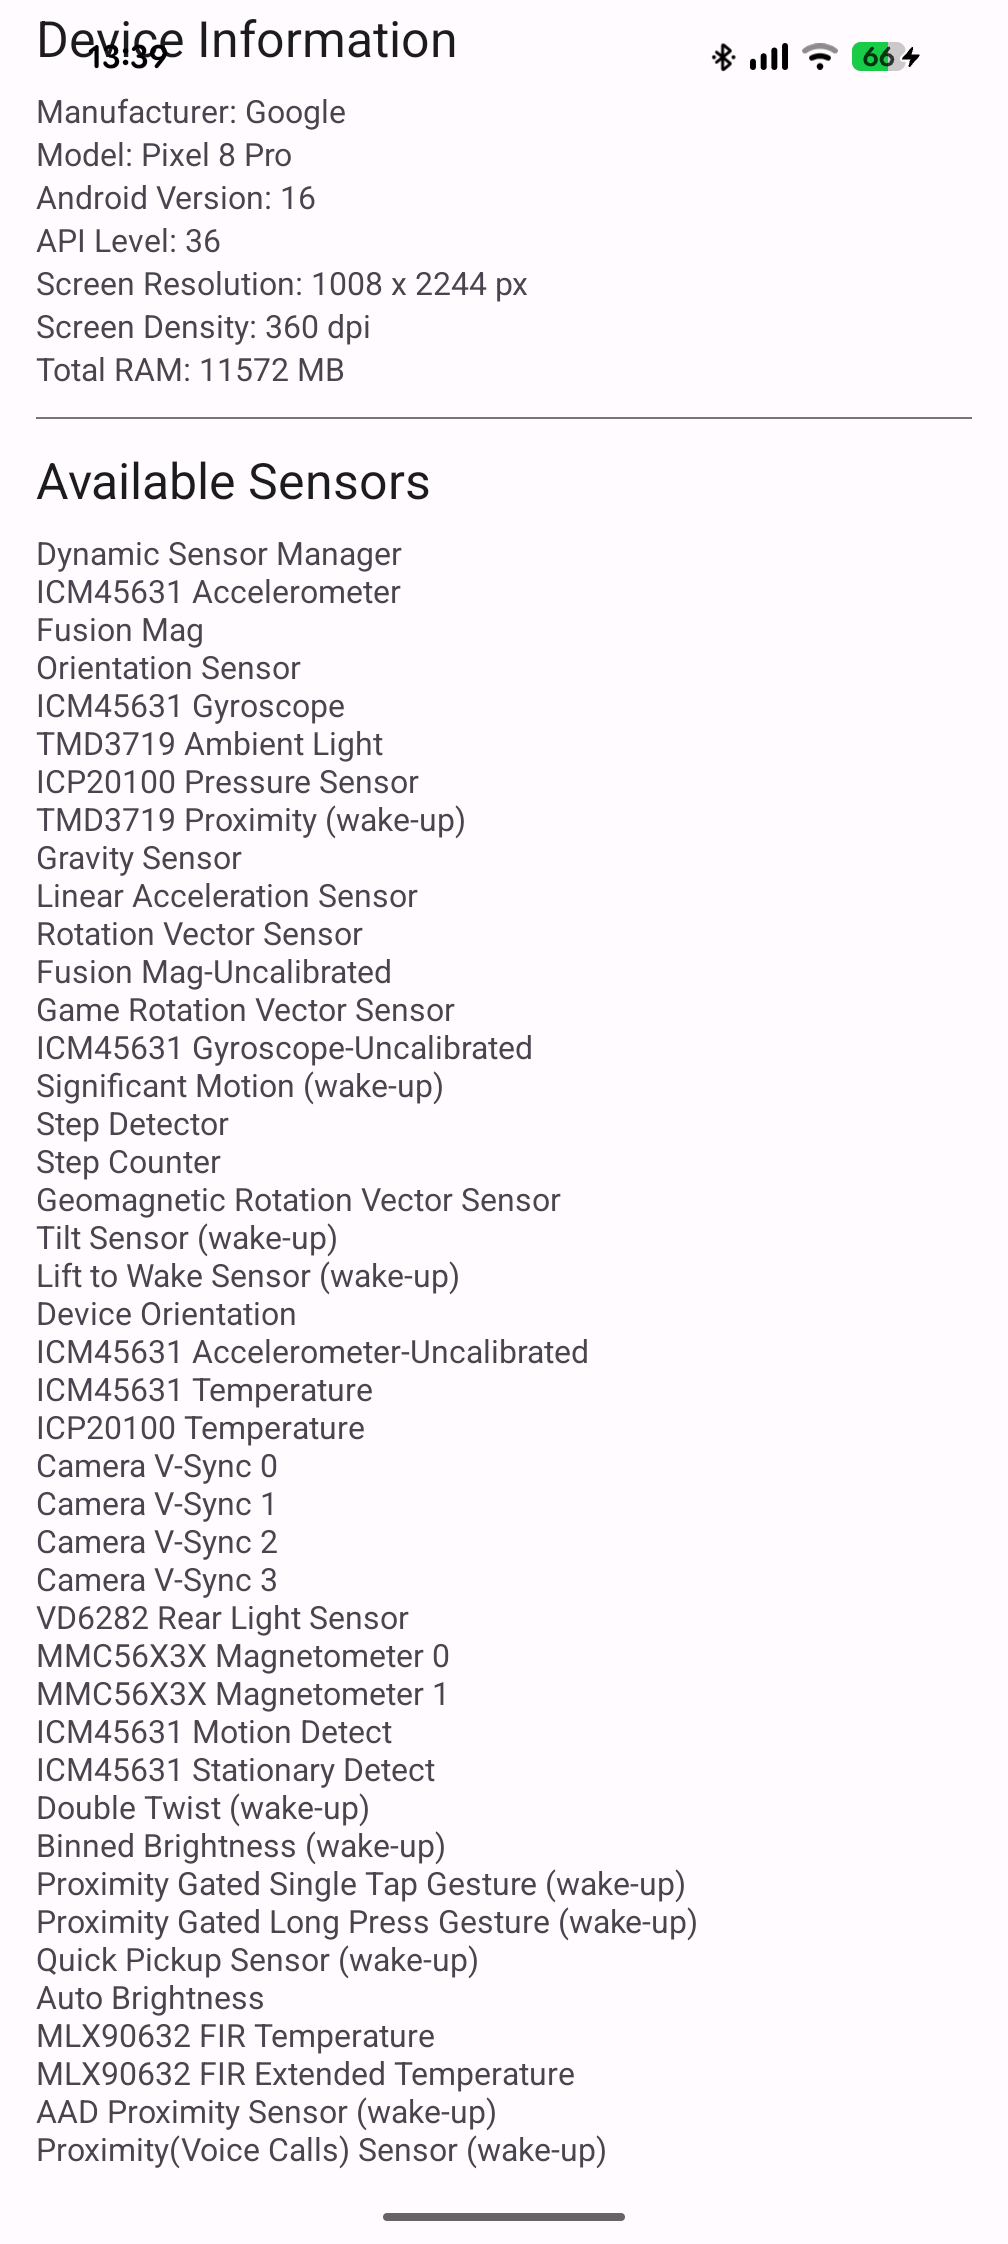
\includegraphics[height=0.75\textheight]{Screenshot_20260612-133922}
    \caption{Output of the Sensor Overview app on a Pixel 8 Pro.}
    \label{fig:screenshot}
\end{figure}

\section{Sensors for Measuring Parkinson's Disease}
Parkinson's disease manifests in motor symptoms such as resting tremor, slowness of movement, rigidity and an
unstable gait. These symptoms can be captured well with the motion sensors
of a smartphone:

\begin{itemize}
    \item Accelerometer
    \item Gyroscope
    \item Linear Acceleration / Gravity Sensor
    \item Rotation Vector / Orientation Sensor
    \item Step Detector / Step Counter
\end{itemize}

The \textbf{accelerometer in combination with the gyroscope} is the best
choice: they directly capture the characteristic resting tremor,
which can be identified with a simple frequency analysis (e.g.\ FFT).
\end{document}
